\section{Дневник отладки}

Изначально я считывал данные как float, но клал их в массив с double, и у меня выходило что два семпла float лежали в одном элементе массива double. Из-за этого во многих песнях процент совпадения был маленьких. Так же это можно увидеть на графике для частоты 40Гц: Он выглядит неестественно, так как звук одной частоты должен представлять синусоиду.

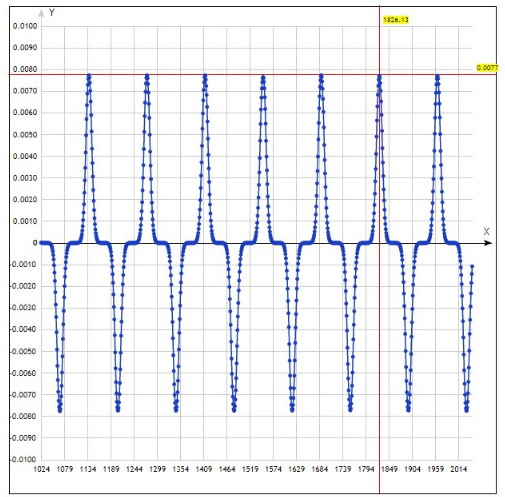
\includegraphics{double.png}

\pagebreak

Но после замены всех переменных с double на float, процент совпадения в песне значительно увеличивается и график приходит в норму.

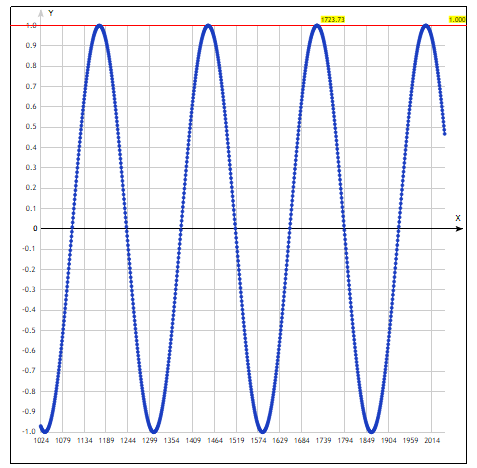
\includegraphics{float.png}  

\pagebreak